\documentclass[twoside]{article}

% Packages required by doxygen
\usepackage{calc}
\usepackage{doxygen}
\usepackage{graphicx}
\usepackage[utf8]{inputenc}
\usepackage{makeidx}
\usepackage{multicol}
\usepackage{multirow}
\usepackage{textcomp}
\usepackage[table]{xcolor}

% Font selection
\usepackage[T1]{fontenc}
\usepackage{mathptmx}
\usepackage[scaled=.90]{helvet}
\usepackage{courier}
\usepackage{amssymb}
\usepackage{sectsty}
\renewcommand{\familydefault}{\sfdefault}
\allsectionsfont{%
  \fontseries{bc}\selectfont%
  \color{darkgray}%
}
\renewcommand{\DoxyLabelFont}{%
  \fontseries{bc}\selectfont%
  \color{darkgray}%
}

% Page & text layout
\usepackage{geometry}
\geometry{%
  a4paper,%
  top=2.5cm,%
  bottom=2.5cm,%
  left=2.5cm,%
  right=2.5cm%
}
\tolerance=750
\hfuzz=15pt
\hbadness=750
\setlength{\emergencystretch}{15pt}
\setlength{\parindent}{0cm}
\setlength{\parskip}{0.2cm}
\makeatletter
\renewcommand{\paragraph}{%
  \@startsection{paragraph}{4}{0ex}{-1.0ex}{1.0ex}{%
    \normalfont\normalsize\bfseries\SS@parafont%
  }%
}
\renewcommand{\subparagraph}{%
  \@startsection{subparagraph}{5}{0ex}{-1.0ex}{1.0ex}{%
    \normalfont\normalsize\bfseries\SS@subparafont%
  }%
}
\makeatother

% Headers & footers
\usepackage{fancyhdr}
\pagestyle{fancyplain}
\fancyhead[LE]{\fancyplain{}{\bfseries\thepage}}
\fancyhead[CE]{\fancyplain{}{}}
\fancyhead[RE]{\fancyplain{}{\bfseries\leftmark}}
\fancyhead[LO]{\fancyplain{}{\bfseries\rightmark}}
\fancyhead[CO]{\fancyplain{}{}}
\fancyhead[RO]{\fancyplain{}{\bfseries\thepage}}
\fancyfoot[LE]{\fancyplain{}{}}
\fancyfoot[CE]{\fancyplain{}{}}
\fancyfoot[RE]{\fancyplain{}{\bfseries\scriptsize Generated on Sat Nov 9 2013 22\-:15\-:20 for Cat Mouse by Doxygen }}
\fancyfoot[LO]{\fancyplain{}{\bfseries\scriptsize Generated on Sat Nov 9 2013 22\-:15\-:20 for Cat Mouse by Doxygen }}
\fancyfoot[CO]{\fancyplain{}{}}
\fancyfoot[RO]{\fancyplain{}{}}
\renewcommand{\footrulewidth}{0.4pt}
\renewcommand{\sectionmark}[1]{%
  \markright{\thesection\ #1}%
}

% Indices & bibliography
\usepackage{natbib}
\usepackage[titles]{tocloft}
\setcounter{tocdepth}{3}
\setcounter{secnumdepth}{5}
\makeindex

% Custom commands
\newcommand{\clearemptydoublepage}{%
  \newpage{\pagestyle{empty}\cleardoublepage}%
}


%===== C O N T E N T S =====

\begin{document}

% Titlepage & ToC
\pagenumbering{roman}
\begin{titlepage}
\vspace*{7cm}
\begin{center}%
{\Large Cat Mouse \\[1ex]\large High Distinction Project for H\-I\-T2302 Object Oriented Programming }\\
\vspace*{1cm}
{\large Generated by Doxygen 1.8.5}\\
\vspace*{0.5cm}
{\small Sat Nov 9 2013 22:15:20}\\
\end{center}
\end{titlepage}
\tableofcontents
\pagenumbering{arabic}

%--- Begin generated contents ---
\section{C++ Decoupled Implementation}
\label{index}\begin{DoxyVersion}{Version}
3 
\end{DoxyVersion}

\section{Class Documentation}
\subsection{Animal Class Reference}
\label{class_animal}\index{Animal@{Animal}}


{\ttfamily \#include $<$Animal.\-h$>$}



Inheritance diagram for Animal\-:
\nopagebreak
\begin{figure}[H]
\begin{center}
\leavevmode
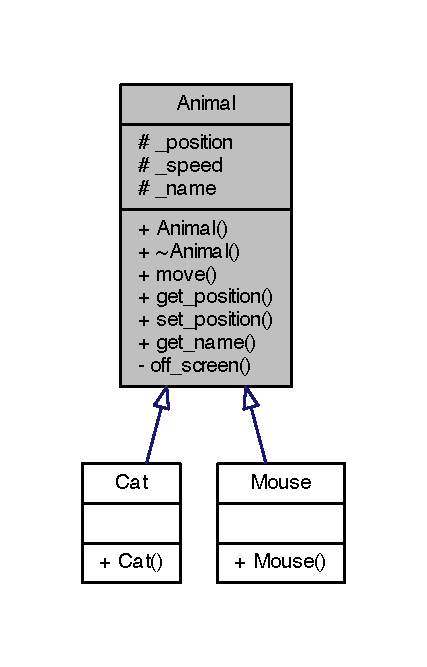
\includegraphics[width=205pt]{class_animal__inherit__graph}
\end{center}
\end{figure}


Collaboration diagram for Animal\-:
\nopagebreak
\begin{figure}[H]
\begin{center}
\leavevmode
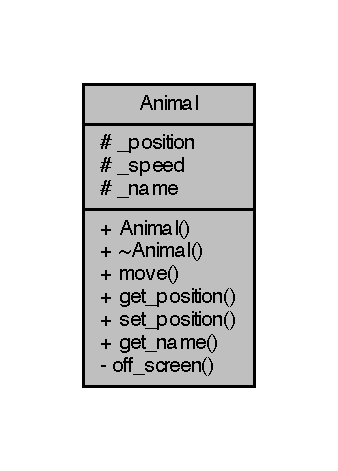
\includegraphics[width=162pt]{class_animal__coll__graph}
\end{center}
\end{figure}
\subsubsection*{Public Member Functions}
\begin{DoxyCompactItemize}
\item 
{\bf Animal} ()
\item 
virtual {\bf $\sim$\-Animal} ()=0
\item 
void {\bf move} ({\bf dirs} dir)
\item 
point2d $\ast$const {\bf get\-\_\-position} ()
\item 
void {\bf set\-\_\-position} (point2d $\ast$new\-Pos)
\item 
string const {\bf get\-\_\-name} ()
\end{DoxyCompactItemize}
\subsubsection*{Protected Attributes}
\begin{DoxyCompactItemize}
\item 
point2d $\ast$ {\bf \-\_\-position}
\item 
const int {\bf \-\_\-speed} = 3
\item 
string {\bf \-\_\-name}
\end{DoxyCompactItemize}
\subsubsection*{Private Member Functions}
\begin{DoxyCompactItemize}
\item 
void {\bf off\-\_\-screen} ()
\end{DoxyCompactItemize}


\subsubsection{Detailed Description}
Defines an abstract, base class for a playable `thing' on the screen which can move around etc. 

Defines class for the general `game' of the cat and mice.

\begin{DoxyAuthor}{Author}
Alex Cummaudo 
\end{DoxyAuthor}
\begin{DoxyDate}{Date}
16 Oct 2013 
\end{DoxyDate}


\subsubsection{Constructor \& Destructor Documentation}
\index{Animal@{Animal}!Animal@{Animal}}
\index{Animal@{Animal}!Animal@{Animal}}
\paragraph[{Animal}]{\setlength{\rightskip}{0pt plus 5cm}Animal\-::\-Animal (
\begin{DoxyParamCaption}
{}
\end{DoxyParamCaption}
)}\label{class_animal_a1e726a49ec952443190ac62dad22353c}


Default constructor for initialising \-\_\-position and \-\_\-speed for all new Animals. 

\index{Animal@{Animal}!$\sim$\-Animal@{$\sim$\-Animal}}
\index{$\sim$\-Animal@{$\sim$\-Animal}!Animal@{Animal}}
\paragraph[{$\sim$\-Animal}]{\setlength{\rightskip}{0pt plus 5cm}Animal\-::$\sim$\-Animal (
\begin{DoxyParamCaption}
{}
\end{DoxyParamCaption}
)\hspace{0.3cm}{\ttfamily [pure virtual]}}\label{class_animal_a85ab5e8d0fa7cc6fa5836d4279fac8ea}


Destructor reliquishes resources created in this class. 



\subsubsection{Member Function Documentation}
\index{Animal@{Animal}!move@{move}}
\index{move@{move}!Animal@{Animal}}
\paragraph[{move}]{\setlength{\rightskip}{0pt plus 5cm}void Animal\-::move (
\begin{DoxyParamCaption}
\item[{{\bf dirs}}]{dir}
\end{DoxyParamCaption}
)}\label{class_animal_af9eb2023be0d8c67b29112a17be11f5d}


Move implementation for a \doxyref{Animal}{p.}{class_animal} to move an animal in a direction at its speed. 


\begin{DoxyParams}{Parameters}
{\em dir} & Direction the animal is told to move in (alters x and y axis position of poisition accordingly) \\
\hline
\end{DoxyParams}
\index{Animal@{Animal}!get\-\_\-position@{get\-\_\-position}}
\index{get\-\_\-position@{get\-\_\-position}!Animal@{Animal}}
\paragraph[{get\-\_\-position}]{\setlength{\rightskip}{0pt plus 5cm}point2d$\ast$ const Animal\-::get\-\_\-position (
\begin{DoxyParamCaption}
{}
\end{DoxyParamCaption}
)}\label{class_animal_a9e307e2b46e3732f0797ed4579467244}
Read property to get the position of the \doxyref{Animal}{p.}{class_animal} \begin{DoxyReturn}{Returns}
Position of the animal 
\end{DoxyReturn}
\index{Animal@{Animal}!set\-\_\-position@{set\-\_\-position}}
\index{set\-\_\-position@{set\-\_\-position}!Animal@{Animal}}
\paragraph[{set\-\_\-position}]{\setlength{\rightskip}{0pt plus 5cm}void Animal\-::set\-\_\-position (
\begin{DoxyParamCaption}
\item[{point2d $\ast$}]{new\-Pos}
\end{DoxyParamCaption}
)}\label{class_animal_aaea75409f44cb02b63b7fbc4a8184197}
Write property to set the position of the \doxyref{Animal}{p.}{class_animal} 
\begin{DoxyParams}{Parameters}
{\em new\-Pos} & New position to set the animal at \\
\hline
\end{DoxyParams}
\index{Animal@{Animal}!get\-\_\-name@{get\-\_\-name}}
\index{get\-\_\-name@{get\-\_\-name}!Animal@{Animal}}
\paragraph[{get\-\_\-name}]{\setlength{\rightskip}{0pt plus 5cm}string const Animal\-::get\-\_\-name (
\begin{DoxyParamCaption}
{}
\end{DoxyParamCaption}
)}\label{class_animal_a6c3b80380c4d16b2f66c69b739dfbf2f}
Readonly property to get the name of the animal \begin{DoxyReturn}{Returns}
Name of the animal 
\end{DoxyReturn}
\index{Animal@{Animal}!off\-\_\-screen@{off\-\_\-screen}}
\index{off\-\_\-screen@{off\-\_\-screen}!Animal@{Animal}}
\paragraph[{off\-\_\-screen}]{\setlength{\rightskip}{0pt plus 5cm}void Animal\-::off\-\_\-screen (
\begin{DoxyParamCaption}
{}
\end{DoxyParamCaption}
)\hspace{0.3cm}{\ttfamily [private]}}\label{class_animal_ab17f87c66cc4d47f8fd1219385a1197a}


Off screen check that prevents any \doxyref{Animal}{p.}{class_animal} from going outside the borders of the screen. 



\subsubsection{Member Data Documentation}
\index{Animal@{Animal}!\-\_\-position@{\-\_\-position}}
\index{\-\_\-position@{\-\_\-position}!Animal@{Animal}}
\paragraph[{\-\_\-position}]{\setlength{\rightskip}{0pt plus 5cm}point2d$\ast$ Animal\-::\-\_\-position\hspace{0.3cm}{\ttfamily [protected]}}\label{class_animal_a12bf4eaa06117fd600c2cd1bd0972aac}


Centrepoint position of the animal. 

\index{Animal@{Animal}!\-\_\-speed@{\-\_\-speed}}
\index{\-\_\-speed@{\-\_\-speed}!Animal@{Animal}}
\paragraph[{\-\_\-speed}]{\setlength{\rightskip}{0pt plus 5cm}const int Animal\-::\-\_\-speed = 3\hspace{0.3cm}{\ttfamily [protected]}}\label{class_animal_aedafd92e6aa3a78449b6a90875e03701}


Speed at which animals move at, set to a value of 3. 

\index{Animal@{Animal}!\-\_\-name@{\-\_\-name}}
\index{\-\_\-name@{\-\_\-name}!Animal@{Animal}}
\paragraph[{\-\_\-name}]{\setlength{\rightskip}{0pt plus 5cm}string Animal\-::\-\_\-name\hspace{0.3cm}{\ttfamily [protected]}}\label{class_animal_af1e4f3632becd0325781b5f028d5ff5e}


Name of animals, overriden by children (i.\-e. `\-Cat' or `\-Mouse') 



The documentation for this class was generated from the following files\-:\begin{DoxyCompactItemize}
\item 
/\-Users/\-Alex/\-Dropbox/\-Swinburne/\-H\-I\-T2302 -\/ O\-O\-P/\-Projects/\-Cat and Mouse/\#1\-\_\-\-Cat\-Mouse\-\_\-\-C++\-\_\-\-D\-E\-Coupled/src/{\bf Animal.\-h}\item 
/\-Users/\-Alex/\-Dropbox/\-Swinburne/\-H\-I\-T2302 -\/ O\-O\-P/\-Projects/\-Cat and Mouse/\#1\-\_\-\-Cat\-Mouse\-\_\-\-C++\-\_\-\-D\-E\-Coupled/src/{\bf Animal.\-cpp}\end{DoxyCompactItemize}

\subsection{Cat Class Reference}
\label{class_cat}\index{Cat@{Cat}}


{\ttfamily \#include $<$Cat\-Mouse.\-hpp$>$}



Inheritance diagram for Cat\-:
\nopagebreak
\begin{figure}[H]
\begin{center}
\leavevmode
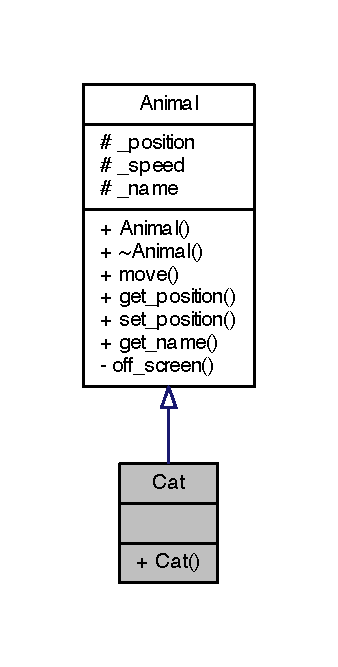
\includegraphics[width=162pt]{class_cat__inherit__graph}
\end{center}
\end{figure}


Collaboration diagram for Cat\-:
\nopagebreak
\begin{figure}[H]
\begin{center}
\leavevmode
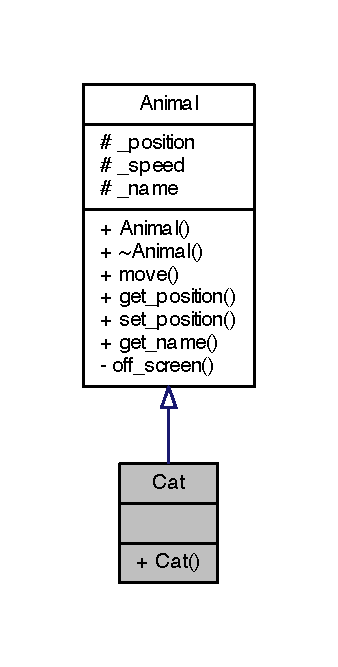
\includegraphics[width=162pt]{class_cat__coll__graph}
\end{center}
\end{figure}
\subsubsection*{Public Member Functions}
\begin{DoxyCompactItemize}
\item 
{\bf Cat} ()
\end{DoxyCompactItemize}
\subsubsection*{Additional Inherited Members}


\subsubsection{Detailed Description}
Defines an class for a playable chaser (i.\-e. the chasing cat) 

\begin{DoxyAuthor}{Author}
Alex Cummaudo 
\end{DoxyAuthor}
\begin{DoxyDate}{Date}
18 Oct 2013 
\end{DoxyDate}


\subsubsection{Constructor \& Destructor Documentation}
\index{Cat@{Cat}!Cat@{Cat}}
\index{Cat@{Cat}!Cat@{Cat}}
\paragraph[{Cat}]{\setlength{\rightskip}{0pt plus 5cm}Cat\-::\-Cat (
\begin{DoxyParamCaption}
{}
\end{DoxyParamCaption}
)}\label{class_cat_adff0d67c4d14c4eeeb35b8daa33ee442}


The default constructor for the cat constructs parent and sets position on lefthand-\/side of screen. 



The documentation for this class was generated from the following file\-:\begin{DoxyCompactItemize}
\item 
/\-Users/\-Alex/\-Dropbox/\-Swinburne/\-H\-I\-T2302 -\/ O\-O\-P/\-Projects/\-Cat and Mouse/\#3\-\_\-\-Cat\-Mouse\-\_\-\-C++\-\_\-\-Coupled/src/{\bf Cat\-Mouse.\-hpp}\end{DoxyCompactItemize}

\subsection{Event Class Reference}
\label{class_event}\index{Event@{Event}}


{\ttfamily \#include $<$Event.\-h$>$}



Collaboration diagram for Event\-:
\nopagebreak
\begin{figure}[H]
\begin{center}
\leavevmode
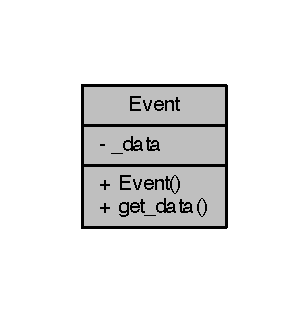
\includegraphics[width=148pt]{class_event__coll__graph}
\end{center}
\end{figure}
\subsubsection*{Public Member Functions}
\begin{DoxyCompactItemize}
\item 
{\bf Event} (map$<$ string, string $>$ data)
\item 
map$<$ string, string $>$ const {\bf get\-\_\-data} ()
\end{DoxyCompactItemize}
\subsubsection*{Private Attributes}
\begin{DoxyCompactItemize}
\item 
map$<$ string, string $>$ {\bf \-\_\-data}
\end{DoxyCompactItemize}


\subsubsection{Detailed Description}
Defines event class of what to pass a view, thereby allowing a link between each view and each model. 

\begin{DoxyAuthor}{Author}
Alex Cummaudo 
\end{DoxyAuthor}
\begin{DoxyDate}{Date}
7 Oct 2013 
\end{DoxyDate}


\subsubsection{Constructor \& Destructor Documentation}
\index{Event@{Event}!Event@{Event}}
\index{Event@{Event}!Event@{Event}}
\paragraph[{Event}]{\setlength{\rightskip}{0pt plus 5cm}Event\-::\-Event (
\begin{DoxyParamCaption}
\item[{map$<$ string, string $>$}]{data}
\end{DoxyParamCaption}
)}\label{class_event_ad16cf2680f59b219dade6053cdbc0a2b}


Constructor for new event object to initialise fields. 


\begin{DoxyParams}{Parameters}
{\em data} & Textual data to insert as data to this event \\
\hline
\end{DoxyParams}


\subsubsection{Member Function Documentation}
\index{Event@{Event}!get\-\_\-data@{get\-\_\-data}}
\index{get\-\_\-data@{get\-\_\-data}!Event@{Event}}
\paragraph[{get\-\_\-data}]{\setlength{\rightskip}{0pt plus 5cm}map$<$string, string$>$ const Event\-::get\-\_\-data (
\begin{DoxyParamCaption}
{}
\end{DoxyParamCaption}
)}\label{class_event_ac2a18b68f3df69b0be35411a5d0abb65}


Readonly property to data. 



\subsubsection{Member Data Documentation}
\index{Event@{Event}!\-\_\-data@{\-\_\-data}}
\index{\-\_\-data@{\-\_\-data}!Event@{Event}}
\paragraph[{\-\_\-data}]{\setlength{\rightskip}{0pt plus 5cm}map$<$string, string$>$ Event\-::\-\_\-data\hspace{0.3cm}{\ttfamily [private]}}\label{class_event_a87c6c24fecb7d60b9a8f3693bd332442}


Textual data contained within the \doxyref{Event}{p.}{class_event}. 



The documentation for this class was generated from the following files\-:\begin{DoxyCompactItemize}
\item 
/\-Users/\-Alex/\-Dropbox/\-Swinburne/\-H\-I\-T2302 -\/ O\-O\-P/\-Projects/\-Cat and Mouse/\#1\-\_\-\-Cat\-Mouse\-\_\-\-C++\-\_\-\-D\-E\-Coupled/src/{\bf Event.\-h}\item 
/\-Users/\-Alex/\-Dropbox/\-Swinburne/\-H\-I\-T2302 -\/ O\-O\-P/\-Projects/\-Cat and Mouse/\#1\-\_\-\-Cat\-Mouse\-\_\-\-C++\-\_\-\-D\-E\-Coupled/src/{\bf Event.\-cpp}\end{DoxyCompactItemize}

\subsection{Event\-Announcer Interface Reference}
\label{class_event_announcer}\index{Event\-Announcer@{Event\-Announcer}}


{\ttfamily \#include $<$Event\-Announcer.\-h$>$}



Inheritance diagram for Event\-Announcer\-:
\nopagebreak
\begin{figure}[H]
\begin{center}
\leavevmode
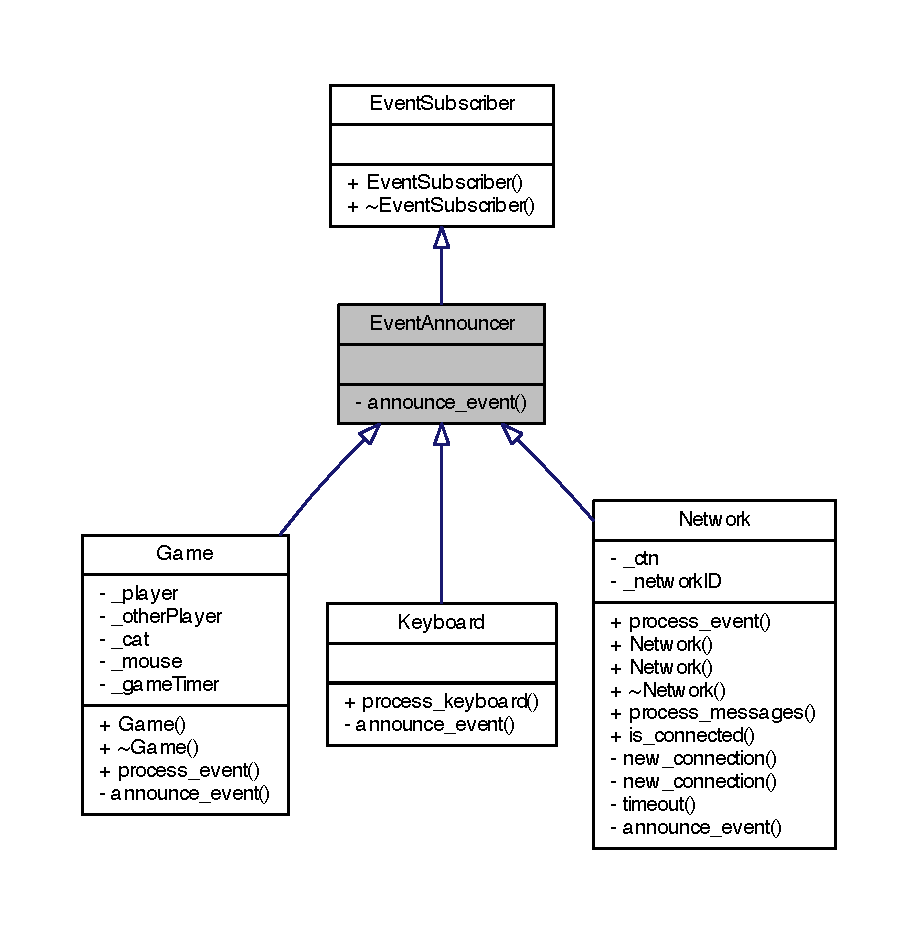
\includegraphics[width=350pt]{class_event_announcer__inherit__graph}
\end{center}
\end{figure}


Collaboration diagram for Event\-Announcer\-:
\nopagebreak
\begin{figure}[H]
\begin{center}
\leavevmode
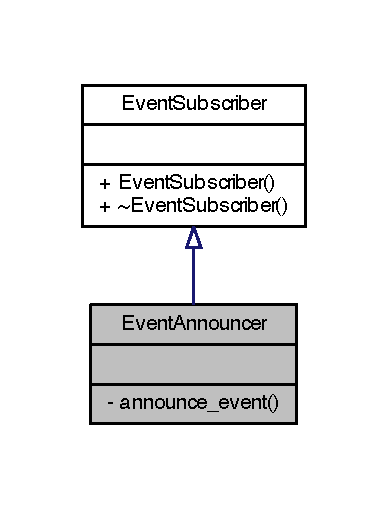
\includegraphics[width=186pt]{class_event_announcer__coll__graph}
\end{center}
\end{figure}
\subsubsection*{Private Member Functions}
\begin{DoxyCompactItemize}
\item 
virtual void {\bf announce\-\_\-event} (string msg)=0
\end{DoxyCompactItemize}
\subsubsection*{Additional Inherited Members}


\subsubsection{Detailed Description}
An pure abstract class that defines all the methods that each announcer of events must implement. 

\begin{DoxyAuthor}{Author}
Alex Cummaudo 
\end{DoxyAuthor}
\begin{DoxyDate}{Date}
7 Oct 2013 
\end{DoxyDate}
\begin{DoxyNote}{Note}
Inherits as virtual so that any users of B\-O\-T\-H Event\-Processors and Event\-Subscribers will avoid diamond inheritance issues. 
\end{DoxyNote}


\subsubsection{Member Function Documentation}
\index{Event\-Announcer@{Event\-Announcer}!announce\-\_\-event@{announce\-\_\-event}}
\index{announce\-\_\-event@{announce\-\_\-event}!EventAnnouncer@{Event\-Announcer}}
\paragraph[{announce\-\_\-event}]{\setlength{\rightskip}{0pt plus 5cm}virtual void Event\-Announcer\-::announce\-\_\-event (
\begin{DoxyParamCaption}
\item[{string}]{msg}
\end{DoxyParamCaption}
)\hspace{0.3cm}{\ttfamily [private]}, {\ttfamily [pure virtual]}}\label{class_event_announcer_a44cb9090f6a15571de9a2f605cd4d898}


Defines that whoever uses this interface must announce events with given a message to the \doxyref{Event\-Manager}{p.}{class_event_manager}. 


\begin{DoxyParams}{Parameters}
{\em msg} & Message to announce when creating an \doxyref{Event}{p.}{class_event} \\
\hline
\end{DoxyParams}


Implemented in {\bf Network} \doxyref{}{p.}{class_network_aa9fa251f3d9901702987a50dd681e4cc}, {\bf Game} \doxyref{}{p.}{class_game_a86e4977f847093fa5d01089bd748beec}, and {\bf Keyboard} \doxyref{}{p.}{class_keyboard_a95fb72c2a1fc6085f8f76b01e95b97ac}.



The documentation for this interface was generated from the following file\-:\begin{DoxyCompactItemize}
\item 
/\-Users/\-Alex/\-Dropbox/\-Swinburne/\-H\-I\-T2302 -\/ O\-O\-P/\-Projects/\-Cat and Mouse/\#1\-\_\-\-Cat\-Mouse\-\_\-\-C++\-\_\-\-D\-E\-Coupled/src/{\bf Event\-Announcer.\-h}\end{DoxyCompactItemize}

\subsection{Event\-Manager Class Reference}
\label{class_event_manager}\index{Event\-Manager@{Event\-Manager}}


{\ttfamily \#include $<$Event\-Manager.\-h$>$}



Collaboration diagram for Event\-Manager\-:
\nopagebreak
\begin{figure}[H]
\begin{center}
\leavevmode
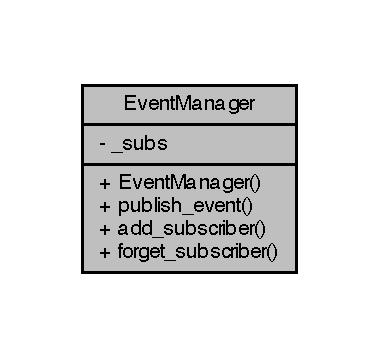
\includegraphics[width=182pt]{class_event_manager__coll__graph}
\end{center}
\end{figure}
\subsubsection*{Public Member Functions}
\begin{DoxyCompactItemize}
\item 
{\bf Event\-Manager} ()
\end{DoxyCompactItemize}
\subsubsection*{Static Public Member Functions}
\begin{DoxyCompactItemize}
\item 
static void {\bf publish\-\_\-event} ({\bf Event} $\ast$e\-Data)
\item 
static void {\bf add\-\_\-subscriber} ({\bf Event\-Subscriber} $\ast$sub)
\item 
static void {\bf forget\-\_\-subscriber} ({\bf Event\-Subscriber} $\ast$sub)
\end{DoxyCompactItemize}
\subsubsection*{Static Private Attributes}
\begin{DoxyCompactItemize}
\item 
static vector$<$ {\bf Event\-Subscriber} $\ast$ $>$ $\ast$ {\bf \-\_\-subs}
\end{DoxyCompactItemize}


\subsubsection{Detailed Description}
Defines \doxyref{Event\-Manager}{p.}{class_event_manager} class which processes each event to each kind of \doxyref{Event\-Processor}{p.}{class_event_processor}. 

\begin{DoxyAuthor}{Author}
Alex Cummaudo 
\end{DoxyAuthor}
\begin{DoxyDate}{Date}
7 Oct 2013 
\end{DoxyDate}
\begin{DoxyNote}{Note}
This is a static member class; so that clients do not need to make an instance of an \doxyref{Event\-Manager}{p.}{class_event_manager} (since there's only ever going to be one processor). Therefore we invoke \doxyref{Event\-Manager}{p.}{class_event_manager} by calling directly on the class (i.\-e. Event\-Manager\-::notify\-\_\-subscribers(event)) 
\end{DoxyNote}


\subsubsection{Constructor \& Destructor Documentation}
\index{Event\-Manager@{Event\-Manager}!Event\-Manager@{Event\-Manager}}
\index{Event\-Manager@{Event\-Manager}!EventManager@{Event\-Manager}}
\paragraph[{Event\-Manager}]{\setlength{\rightskip}{0pt plus 5cm}Event\-Manager\-::\-Event\-Manager (
\begin{DoxyParamCaption}
{}
\end{DoxyParamCaption}
)}\label{class_event_manager_a89099b22114f158b5c530edfea52371d}


Constructor initialises \-\_\-subs vector. 



\subsubsection{Member Function Documentation}
\index{Event\-Manager@{Event\-Manager}!publish\-\_\-event@{publish\-\_\-event}}
\index{publish\-\_\-event@{publish\-\_\-event}!EventManager@{Event\-Manager}}
\paragraph[{publish\-\_\-event}]{\setlength{\rightskip}{0pt plus 5cm}void Event\-Manager\-::publish\-\_\-event (
\begin{DoxyParamCaption}
\item[{{\bf Event} $\ast$}]{e\-Data}
\end{DoxyParamCaption}
)\hspace{0.3cm}{\ttfamily [static]}}\label{class_event_manager_aabfb6a74c877b0b1a6cc208282015d00}


Processes the event for each kind subscriber who publishes events (i.\-e. Event\-Processors O\-N\-L\-Y!) 


\begin{DoxyParams}{Parameters}
{\em e\-Data} & \doxyref{Event}{p.}{class_event} to publish to all Event\-Processors \\
\hline
\end{DoxyParams}
\index{Event\-Manager@{Event\-Manager}!add\-\_\-subscriber@{add\-\_\-subscriber}}
\index{add\-\_\-subscriber@{add\-\_\-subscriber}!EventManager@{Event\-Manager}}
\paragraph[{add\-\_\-subscriber}]{\setlength{\rightskip}{0pt plus 5cm}void Event\-Manager\-::add\-\_\-subscriber (
\begin{DoxyParamCaption}
\item[{{\bf Event\-Subscriber} $\ast$}]{sub}
\end{DoxyParamCaption}
)\hspace{0.3cm}{\ttfamily [static]}}\label{class_event_manager_aad31c655d35869c7265f442f0a056d07}


Adds a subscriber to the \-\_\-subs vector. 


\begin{DoxyParams}{Parameters}
{\em sub} & Subscriber to manage \\
\hline
\end{DoxyParams}
\index{Event\-Manager@{Event\-Manager}!forget\-\_\-subscriber@{forget\-\_\-subscriber}}
\index{forget\-\_\-subscriber@{forget\-\_\-subscriber}!EventManager@{Event\-Manager}}
\paragraph[{forget\-\_\-subscriber}]{\setlength{\rightskip}{0pt plus 5cm}void Event\-Manager\-::forget\-\_\-subscriber (
\begin{DoxyParamCaption}
\item[{{\bf Event\-Subscriber} $\ast$}]{sub}
\end{DoxyParamCaption}
)\hspace{0.3cm}{\ttfamily [static]}}\label{class_event_manager_af8aa888585327e7f5cb14fa44565cc01}


Removes a subscriber to the \-\_\-subs vector. 


\begin{DoxyParams}{Parameters}
{\em sub} & Subscriber to forget \\
\hline
\end{DoxyParams}


\subsubsection{Member Data Documentation}
\index{Event\-Manager@{Event\-Manager}!\-\_\-subs@{\-\_\-subs}}
\index{\-\_\-subs@{\-\_\-subs}!EventManager@{Event\-Manager}}
\paragraph[{\-\_\-subs}]{\setlength{\rightskip}{0pt plus 5cm}vector$<$ {\bf Event\-Subscriber} $\ast$ $>$ $\ast$ Event\-Manager\-::\-\_\-subs\hspace{0.3cm}{\ttfamily [static]}, {\ttfamily [private]}}\label{class_event_manager_a9e5d9ebb85a1c4c8689c3074661481be}


Declare subscribers (who process or announce events) vector. 



The documentation for this class was generated from the following files\-:\begin{DoxyCompactItemize}
\item 
/\-Users/\-Alex/\-Dropbox/\-Swinburne/\-H\-I\-T2302 -\/ O\-O\-P/\-Projects/\-Cat and Mouse/\#1\-\_\-\-Cat\-Mouse\-\_\-\-C++\-\_\-\-D\-E\-Coupled/src/{\bf Event\-Manager.\-h}\item 
/\-Users/\-Alex/\-Dropbox/\-Swinburne/\-H\-I\-T2302 -\/ O\-O\-P/\-Projects/\-Cat and Mouse/\#1\-\_\-\-Cat\-Mouse\-\_\-\-C++\-\_\-\-D\-E\-Coupled/src/{\bf Event\-Manager.\-cpp}\end{DoxyCompactItemize}

\subsection{Event\-Processor Interface Reference}
\label{class_event_processor}\index{Event\-Processor@{Event\-Processor}}


{\ttfamily \#include $<$Event\-Processor.\-h$>$}



Inheritance diagram for Event\-Processor\-:
\nopagebreak
\begin{figure}[H]
\begin{center}
\leavevmode
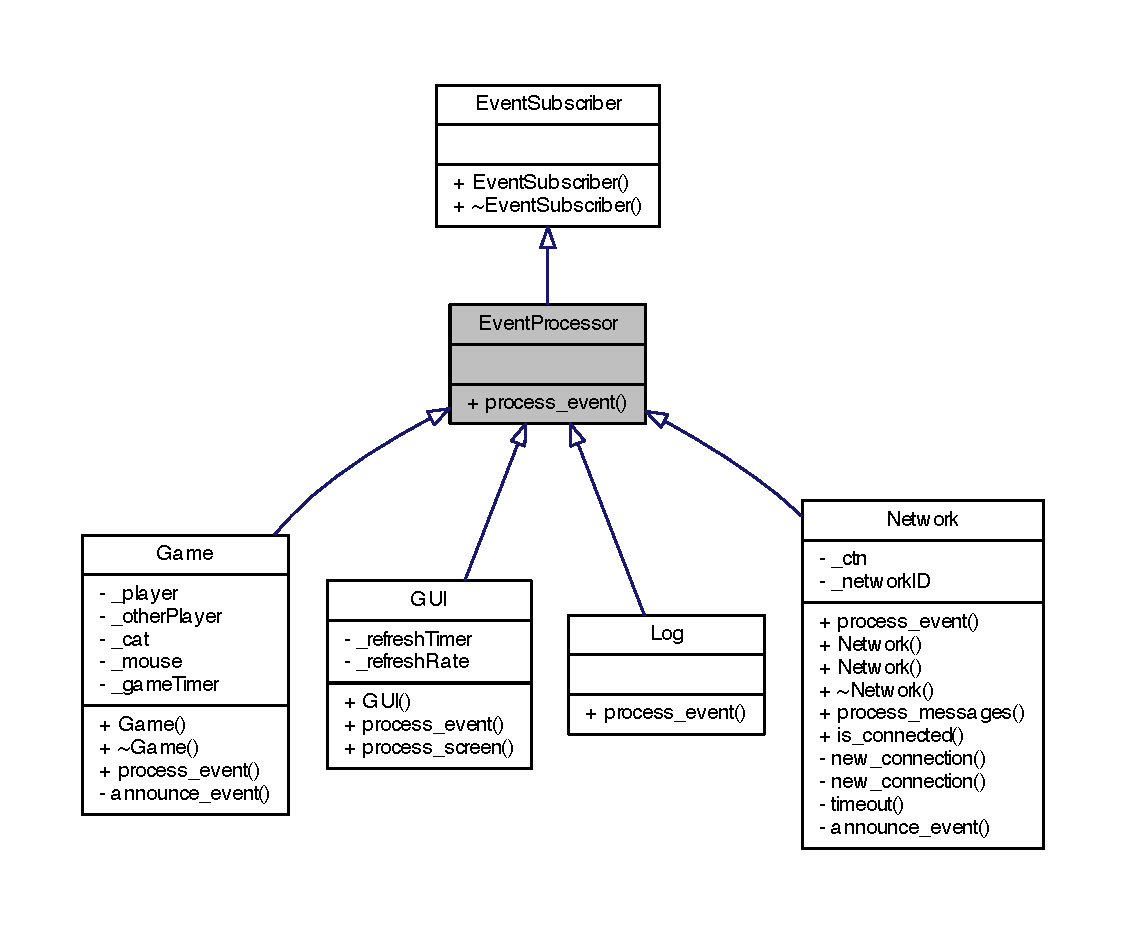
\includegraphics[width=350pt]{class_event_processor__inherit__graph}
\end{center}
\end{figure}


Collaboration diagram for Event\-Processor\-:
\nopagebreak
\begin{figure}[H]
\begin{center}
\leavevmode
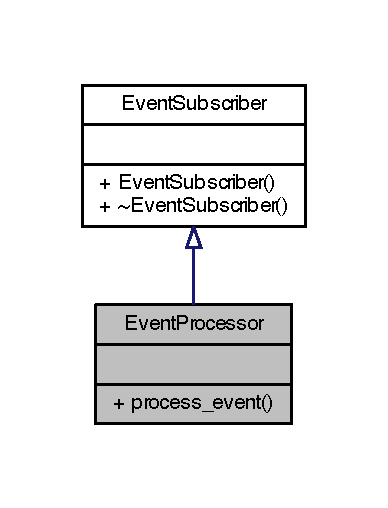
\includegraphics[width=186pt]{class_event_processor__coll__graph}
\end{center}
\end{figure}
\subsubsection*{Public Member Functions}
\begin{DoxyCompactItemize}
\item 
virtual void {\bf process\-\_\-event} ({\bf Event} $\ast$e\-Data)=0
\end{DoxyCompactItemize}


\subsubsection{Detailed Description}
An pure abstract class that defines all the methods that each processor of events must implement. 

\begin{DoxyAuthor}{Author}
Alex Cummaudo 
\end{DoxyAuthor}
\begin{DoxyDate}{Date}
7 Oct 2013 
\end{DoxyDate}
\begin{DoxyNote}{Note}
Inherits as virtual so that any users of B\-O\-T\-H Event\-Processors and Event\-Subscribers will avoid diamond inheritance issues. 
\end{DoxyNote}


\subsubsection{Member Function Documentation}
\index{Event\-Processor@{Event\-Processor}!process\-\_\-event@{process\-\_\-event}}
\index{process\-\_\-event@{process\-\_\-event}!EventProcessor@{Event\-Processor}}
\paragraph[{process\-\_\-event}]{\setlength{\rightskip}{0pt plus 5cm}virtual void Event\-Processor\-::process\-\_\-event (
\begin{DoxyParamCaption}
\item[{{\bf Event} $\ast$}]{e\-Data}
\end{DoxyParamCaption}
)\hspace{0.3cm}{\ttfamily [pure virtual]}}\label{class_event_processor_a20ce019a16fcf8ba67b6547750bf6655}


Defines that whoever uses this interface must process an event in anyway with the given \doxyref{Event}{p.}{class_event}. 


\begin{DoxyParams}{Parameters}
{\em e\-Data} & \doxyref{Event}{p.}{class_event} Data to process \\
\hline
\end{DoxyParams}


Implemented in {\bf Game} \doxyref{}{p.}{class_game_a2651e0c33b4e247719d81cba4bc9e6d8}, {\bf G\-U\-I} \doxyref{}{p.}{class_g_u_i_a1d1b90dd1d77ccc97ce2861359767a20}, {\bf Network} \doxyref{}{p.}{class_network_a2b53d4aa5ca44868b4437a11fe18da97}, and {\bf Log} \doxyref{}{p.}{class_log_a5be2a1f651af3de38cf26a6a84567f51}.



The documentation for this interface was generated from the following file\-:\begin{DoxyCompactItemize}
\item 
/\-Users/\-Alex/\-Dropbox/\-Swinburne/\-H\-I\-T2302 -\/ O\-O\-P/\-Projects/\-Cat and Mouse/\#1\-\_\-\-Cat\-Mouse\-\_\-\-C++\-\_\-\-D\-E\-Coupled/src/{\bf Event\-Processor.\-h}\end{DoxyCompactItemize}

\subsection{Event\-Subscriber Interface Reference}
\label{class_event_subscriber}\index{Event\-Subscriber@{Event\-Subscriber}}


{\ttfamily \#include $<$Event\-Subscriber.\-h$>$}



Inheritance diagram for Event\-Subscriber\-:
\nopagebreak
\begin{figure}[H]
\begin{center}
\leavevmode
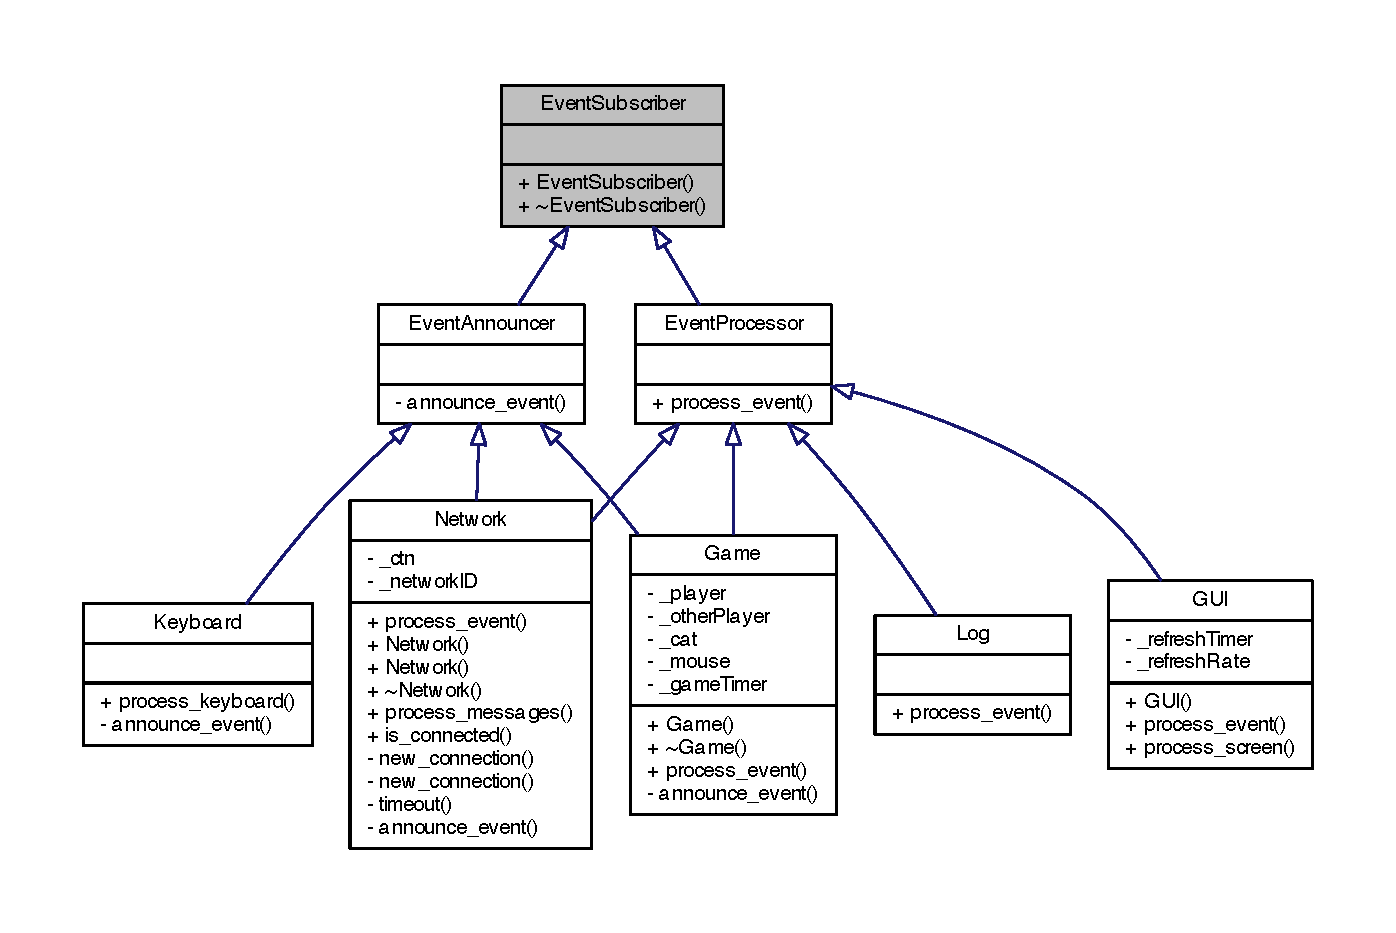
\includegraphics[width=350pt]{class_event_subscriber__inherit__graph}
\end{center}
\end{figure}


Collaboration diagram for Event\-Subscriber\-:
\nopagebreak
\begin{figure}[H]
\begin{center}
\leavevmode
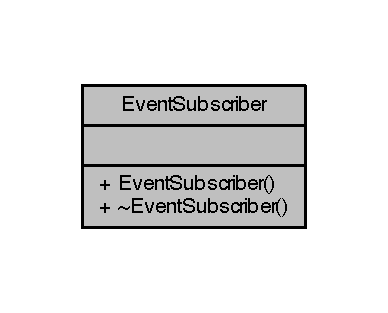
\includegraphics[width=186pt]{class_event_subscriber__coll__graph}
\end{center}
\end{figure}
\subsubsection*{Public Member Functions}
\begin{DoxyCompactItemize}
\item 
{\bf Event\-Subscriber} ()
\item 
virtual {\bf $\sim$\-Event\-Subscriber} ()
\end{DoxyCompactItemize}


\subsubsection{Detailed Description}
Acts as a parent to subscribers and announcers so that the \doxyref{Event}{p.}{class_event} manager knows what to manager (i.\-e. both Announcers and Processors, and this allows this relationship to occur via inheritance) 

\begin{DoxyAuthor}{Author}
Alex Cummaudo 
\end{DoxyAuthor}
\begin{DoxyDate}{Date}
7 Oct 2013 
\end{DoxyDate}


\subsubsection{Constructor \& Destructor Documentation}
\index{Event\-Subscriber@{Event\-Subscriber}!Event\-Subscriber@{Event\-Subscriber}}
\index{Event\-Subscriber@{Event\-Subscriber}!EventSubscriber@{Event\-Subscriber}}
\paragraph[{Event\-Subscriber}]{\setlength{\rightskip}{0pt plus 5cm}Event\-Subscriber\-::\-Event\-Subscriber (
\begin{DoxyParamCaption}
{}
\end{DoxyParamCaption}
)}\label{class_event_subscriber_aedef374acbc811e88f526dd20e86e609}


To dynamically add event subscribers to the \doxyref{Event\-Manager}{p.}{class_event_manager} on creation, the \doxyref{Event\-Subscriber}{p.}{class_event_subscriber} constructor does this for us. 

\index{Event\-Subscriber@{Event\-Subscriber}!$\sim$\-Event\-Subscriber@{$\sim$\-Event\-Subscriber}}
\index{$\sim$\-Event\-Subscriber@{$\sim$\-Event\-Subscriber}!EventSubscriber@{Event\-Subscriber}}
\paragraph[{$\sim$\-Event\-Subscriber}]{\setlength{\rightskip}{0pt plus 5cm}virtual Event\-Subscriber\-::$\sim$\-Event\-Subscriber (
\begin{DoxyParamCaption}
{}
\end{DoxyParamCaption}
)\hspace{0.3cm}{\ttfamily [virtual]}}\label{class_event_subscriber_a04961ec9f1f75657df312524212bcedc}


To make \doxyref{Event\-Subscriber}{p.}{class_event_subscriber} polymorphic, make a virtual destructor---this will allow for dynamic casting in the \doxyref{Event\-Manager}{p.}{class_event_manager}. On invocation, the \doxyref{Event\-Manager}{p.}{class_event_manager} will forget about this subscriber. 



The documentation for this interface was generated from the following file\-:\begin{DoxyCompactItemize}
\item 
/\-Users/\-Alex/\-Dropbox/\-Swinburne/\-H\-I\-T2302 -\/ O\-O\-P/\-Projects/\-Cat and Mouse/\#1\-\_\-\-Cat\-Mouse\-\_\-\-C++\-\_\-\-D\-E\-Coupled/src/{\bf Event\-Subscriber.\-h}\end{DoxyCompactItemize}

\subsection{Game Class Reference}
\label{class_game}\index{Game@{Game}}


{\ttfamily \#include $<$Game.\-h$>$}



Inheritance diagram for Game\-:
\nopagebreak
\begin{figure}[H]
\begin{center}
\leavevmode
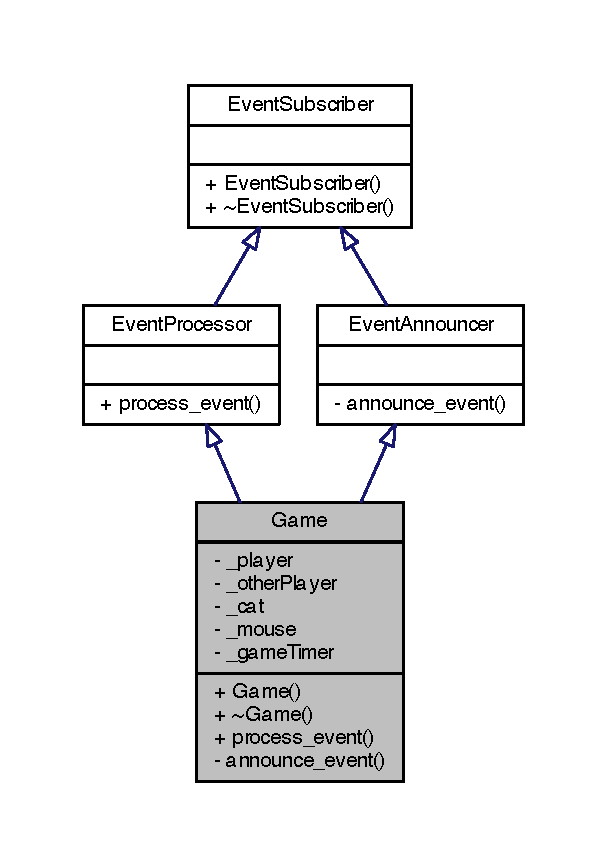
\includegraphics[width=291pt]{class_game__inherit__graph}
\end{center}
\end{figure}


Collaboration diagram for Game\-:
\nopagebreak
\begin{figure}[H]
\begin{center}
\leavevmode
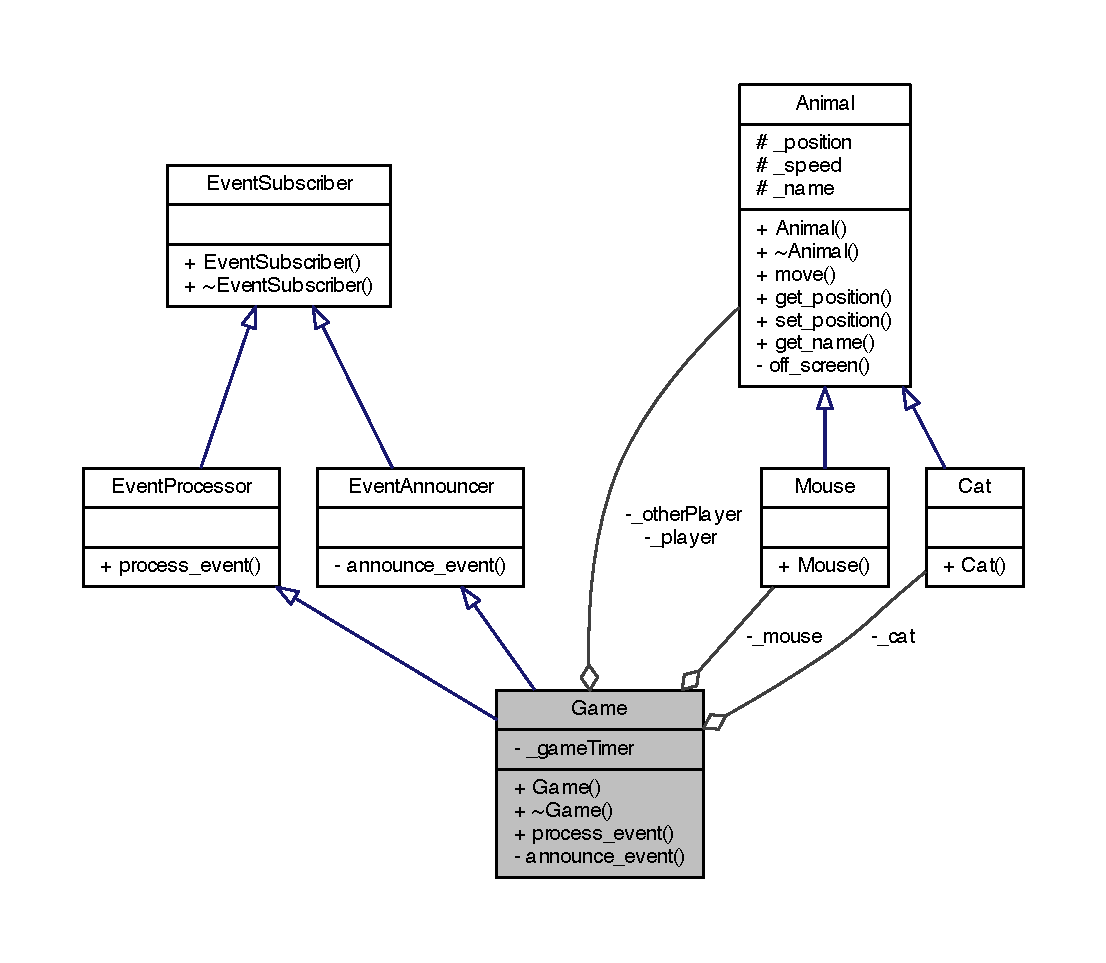
\includegraphics[width=350pt]{class_game__coll__graph}
\end{center}
\end{figure}
\subsubsection*{Public Member Functions}
\begin{DoxyCompactItemize}
\item 
{\bf Game} (bool as\-Cat)
\item 
{\bf $\sim$\-Game} ()
\item 
virtual void {\bf process\-\_\-event} ({\bf Event} $\ast$e\-Data)
\end{DoxyCompactItemize}
\subsubsection*{Private Member Functions}
\begin{DoxyCompactItemize}
\item 
virtual void {\bf announce\-\_\-event} (string msg)
\end{DoxyCompactItemize}
\subsubsection*{Private Attributes}
\begin{DoxyCompactItemize}
\item 
{\bf Animal} $\ast$ {\bf \-\_\-player}
\item 
{\bf Animal} $\ast$ {\bf \-\_\-other\-Player}
\item 
{\bf Cat} $\ast$ {\bf \-\_\-cat}
\item 
{\bf Mouse} $\ast$ {\bf \-\_\-mouse}
\item 
timer {\bf \-\_\-game\-Timer}
\end{DoxyCompactItemize}


\subsubsection{Detailed Description}
Defines class for the general `game' of the cat and mice. 

\begin{DoxyAuthor}{Author}
Alex Cummaudo 
\end{DoxyAuthor}
\begin{DoxyDate}{Date}
16 Oct 2013 
\end{DoxyDate}


\subsubsection{Constructor \& Destructor Documentation}
\index{Game@{Game}!Game@{Game}}
\index{Game@{Game}!Game@{Game}}
\paragraph[{Game}]{\setlength{\rightskip}{0pt plus 5cm}Game\-::\-Game (
\begin{DoxyParamCaption}
\item[{bool}]{as\-Cat}
\end{DoxyParamCaption}
)}\label{class_game_a2605d0d30be2fa6a5c7cad7565aaeabe}


On construction of a game, a cat and a mouse will be created---if the as\-Cat is true, player references the cat, else it will reference the mouse. 


\begin{DoxyParams}{Parameters}
{\em as\-Cat} & Where true, the game initialises the player as the cat, with the other player as the mouse. \\
\hline
\end{DoxyParams}
\index{Game@{Game}!$\sim$\-Game@{$\sim$\-Game}}
\index{$\sim$\-Game@{$\sim$\-Game}!Game@{Game}}
\paragraph[{$\sim$\-Game}]{\setlength{\rightskip}{0pt plus 5cm}Game\-::$\sim$\-Game (
\begin{DoxyParamCaption}
{}
\end{DoxyParamCaption}
)}\label{class_game_ae3d112ca6e0e55150d2fdbc704474530}


Destructor reliquishes resources created in this class. 



\subsubsection{Member Function Documentation}
\index{Game@{Game}!process\-\_\-event@{process\-\_\-event}}
\index{process\-\_\-event@{process\-\_\-event}!Game@{Game}}
\paragraph[{process\-\_\-event}]{\setlength{\rightskip}{0pt plus 5cm}void Game\-::process\-\_\-event (
\begin{DoxyParamCaption}
\item[{{\bf Event} $\ast$}]{e\-Data}
\end{DoxyParamCaption}
)\hspace{0.3cm}{\ttfamily [virtual]}}\label{class_game_a2651e0c33b4e247719d81cba4bc9e6d8}


Recieves events from the \doxyref{Event\-Manager}{p.}{class_event_manager} to set the coordinates of the players to either a specified location (\-\_\-other\-Player) or to move the \-\_\-player according to key events. 


\begin{DoxyParams}{Parameters}
{\em e\-Data} & \doxyref{Event}{p.}{class_event} Data to process \\
\hline
\end{DoxyParams}


Implements {\bf Event\-Processor} \doxyref{}{p.}{class_event_processor_a20ce019a16fcf8ba67b6547750bf6655}.

\index{Game@{Game}!announce\-\_\-event@{announce\-\_\-event}}
\index{announce\-\_\-event@{announce\-\_\-event}!Game@{Game}}
\paragraph[{announce\-\_\-event}]{\setlength{\rightskip}{0pt plus 5cm}void Game\-::announce\-\_\-event (
\begin{DoxyParamCaption}
\item[{string}]{msg}
\end{DoxyParamCaption}
)\hspace{0.3cm}{\ttfamily [private]}, {\ttfamily [virtual]}}\label{class_game_a86e4977f847093fa5d01089bd748beec}


Announces that the player moved (called by key\-\_\-check on a key move) to all of \doxyref{Event\-Manager}{p.}{class_event_manager}'s Event\-Processors---i.\-e. to announce updates of the model. 


\begin{DoxyParams}{Parameters}
{\em msg} & Message to announce \\
\hline
\end{DoxyParams}


Implements {\bf Event\-Announcer} \doxyref{}{p.}{class_event_announcer_a44cb9090f6a15571de9a2f605cd4d898}.



\subsubsection{Member Data Documentation}
\index{Game@{Game}!\-\_\-player@{\-\_\-player}}
\index{\-\_\-player@{\-\_\-player}!Game@{Game}}
\paragraph[{\-\_\-player}]{\setlength{\rightskip}{0pt plus 5cm}{\bf Animal}$\ast$ Game\-::\-\_\-player\hspace{0.3cm}{\ttfamily [private]}}\label{class_game_a33cf560b060565842b8127a9867d64d5}


Player of the game (person controlling the game) 

\index{Game@{Game}!\-\_\-other\-Player@{\-\_\-other\-Player}}
\index{\-\_\-other\-Player@{\-\_\-other\-Player}!Game@{Game}}
\paragraph[{\-\_\-other\-Player}]{\setlength{\rightskip}{0pt plus 5cm}{\bf Animal}$\ast$ Game\-::\-\_\-other\-Player\hspace{0.3cm}{\ttfamily [private]}}\label{class_game_a5131619bab9ae76ee9289d2fdcd9a14c}


Other player in the game (other person controlling enemy) 

\index{Game@{Game}!\-\_\-cat@{\-\_\-cat}}
\index{\-\_\-cat@{\-\_\-cat}!Game@{Game}}
\paragraph[{\-\_\-cat}]{\setlength{\rightskip}{0pt plus 5cm}{\bf Cat}$\ast$ Game\-::\-\_\-cat\hspace{0.3cm}{\ttfamily [private]}}\label{class_game_a433c454efcf31e54d98a2aa81d4f6801}


\doxyref{Cat}{p.}{class_cat} (chaser) of the game. 

\index{Game@{Game}!\-\_\-mouse@{\-\_\-mouse}}
\index{\-\_\-mouse@{\-\_\-mouse}!Game@{Game}}
\paragraph[{\-\_\-mouse}]{\setlength{\rightskip}{0pt plus 5cm}{\bf Mouse}$\ast$ Game\-::\-\_\-mouse\hspace{0.3cm}{\ttfamily [private]}}\label{class_game_a8e51ead264380e60e29db6bf1d239f36}


\doxyref{Mouse}{p.}{class_mouse} (chasee) of the game. 

\index{Game@{Game}!\-\_\-game\-Timer@{\-\_\-game\-Timer}}
\index{\-\_\-game\-Timer@{\-\_\-game\-Timer}!Game@{Game}}
\paragraph[{\-\_\-game\-Timer}]{\setlength{\rightskip}{0pt plus 5cm}timer Game\-::\-\_\-game\-Timer\hspace{0.3cm}{\ttfamily [private]}}\label{class_game_a1e8cb33307304fe85e3efaa7d27132c0}


Ingame-\/timer to keep track of how long game has gone for. 



The documentation for this class was generated from the following files\-:\begin{DoxyCompactItemize}
\item 
/\-Users/\-Alex/\-Dropbox/\-Swinburne/\-H\-I\-T2302 -\/ O\-O\-P/\-Projects/\-Cat and Mouse/\#1\-\_\-\-Cat\-Mouse\-\_\-\-C++\-\_\-\-D\-E\-Coupled/src/{\bf Game.\-h}\item 
/\-Users/\-Alex/\-Dropbox/\-Swinburne/\-H\-I\-T2302 -\/ O\-O\-P/\-Projects/\-Cat and Mouse/\#1\-\_\-\-Cat\-Mouse\-\_\-\-C++\-\_\-\-D\-E\-Coupled/src/{\bf Game.\-cpp}\end{DoxyCompactItemize}

\subsection{G\-U\-I Class Reference}
\label{class_g_u_i}\index{G\-U\-I@{G\-U\-I}}


{\ttfamily \#include $<$G\-U\-I.\-h$>$}



Collaboration diagram for G\-U\-I\-:
\nopagebreak
\begin{figure}[H]
\begin{center}
\leavevmode
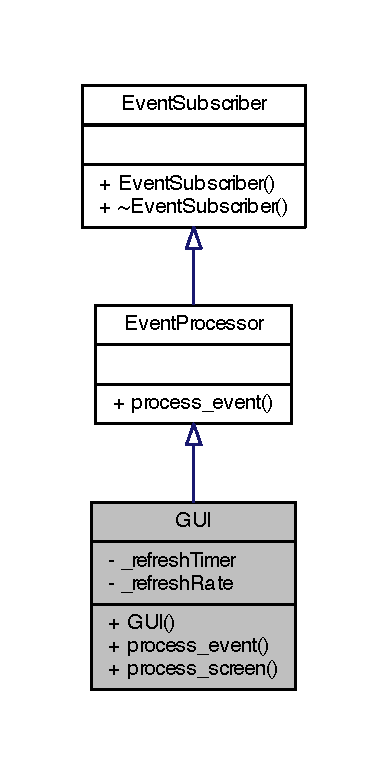
\includegraphics[width=178pt]{class_g_u_i__coll__graph}
\end{center}
\end{figure}
\subsubsection*{Public Member Functions}
\begin{DoxyCompactItemize}
\item 
{\bf G\-U\-I} (float ref\-Rate)
\item 
void {\bf process\-\_\-screen} ()
\item 
void {\bf draw\-\_\-animal} ({\bf Animal} $\ast$animal)
\end{DoxyCompactItemize}
\subsubsection*{Private Attributes}
\begin{DoxyCompactItemize}
\item 
timer {\bf \-\_\-refresh\-Timer}
\item 
float {\bf \-\_\-refresh\-Rate}
\end{DoxyCompactItemize}


\subsubsection{Detailed Description}
Provides \doxyref{G\-U\-I}{p.}{class_g_u_i} View for the game to display the game on in a graphics window. 

\begin{DoxyAuthor}{Author}
Alex Cummaudo 
\end{DoxyAuthor}
\begin{DoxyDate}{Date}
2 Nov 2013 
\end{DoxyDate}


\subsubsection{Constructor \& Destructor Documentation}
\index{G\-U\-I@{G\-U\-I}!G\-U\-I@{G\-U\-I}}
\index{G\-U\-I@{G\-U\-I}!GUI@{G\-U\-I}}
\paragraph[{G\-U\-I}]{\setlength{\rightskip}{0pt plus 5cm}G\-U\-I\-::\-G\-U\-I (
\begin{DoxyParamCaption}
\item[{float}]{ref\-Rate}
\end{DoxyParamCaption}
)}\label{class_g_u_i_a371321c2223659573ebd5b693ea839a8}


Constructor for \doxyref{G\-U\-I}{p.}{class_g_u_i} view creates a graphics window for Swin\-Game. 



\subsubsection{Member Function Documentation}
\index{G\-U\-I@{G\-U\-I}!process\-\_\-screen@{process\-\_\-screen}}
\index{process\-\_\-screen@{process\-\_\-screen}!GUI@{G\-U\-I}}
\paragraph[{process\-\_\-screen}]{\setlength{\rightskip}{0pt plus 5cm}void G\-U\-I\-::process\-\_\-screen (
\begin{DoxyParamCaption}
{}
\end{DoxyParamCaption}
)}\label{class_g_u_i_abb478359b6d62cabce2839c950afbf68}


Clears and refreshes the screen by the time given in reset timer. 

\index{G\-U\-I@{G\-U\-I}!draw\-\_\-animal@{draw\-\_\-animal}}
\index{draw\-\_\-animal@{draw\-\_\-animal}!GUI@{G\-U\-I}}
\paragraph[{draw\-\_\-animal}]{\setlength{\rightskip}{0pt plus 5cm}void G\-U\-I\-::draw\-\_\-animal (
\begin{DoxyParamCaption}
\item[{{\bf Animal} $\ast$}]{animal}
\end{DoxyParamCaption}
)}\label{class_g_u_i_ab2f961bd44c1801f3a5f747a39d6ca43}


Draws the given animal to the screen. 


\begin{DoxyParams}{Parameters}
{\em animal} & \doxyref{Animal}{p.}{class_animal} to draw to the screen \\
\hline
\end{DoxyParams}


\subsubsection{Member Data Documentation}
\index{G\-U\-I@{G\-U\-I}!\-\_\-refresh\-Timer@{\-\_\-refresh\-Timer}}
\index{\-\_\-refresh\-Timer@{\-\_\-refresh\-Timer}!GUI@{G\-U\-I}}
\paragraph[{\-\_\-refresh\-Timer}]{\setlength{\rightskip}{0pt plus 5cm}timer G\-U\-I\-::\-\_\-refresh\-Timer\hspace{0.3cm}{\ttfamily [private]}}\label{class_g_u_i_a10617cc2306e5318fa1d89cef9ee208b}
Timer used to refresh the screen at the by clearing the screen and resetting at refresh\-Rate given \index{G\-U\-I@{G\-U\-I}!\-\_\-refresh\-Rate@{\-\_\-refresh\-Rate}}
\index{\-\_\-refresh\-Rate@{\-\_\-refresh\-Rate}!GUI@{G\-U\-I}}
\paragraph[{\-\_\-refresh\-Rate}]{\setlength{\rightskip}{0pt plus 5cm}float G\-U\-I\-::\-\_\-refresh\-Rate\hspace{0.3cm}{\ttfamily [private]}}\label{class_g_u_i_a4d1f915c03268ce7c9e2896ec82aa83e}


Seconds to refresh the screen at. 



The documentation for this class was generated from the following files\-:\begin{DoxyCompactItemize}
\item 
/\-Users/\-Alex/\-Dropbox/\-Swinburne/\-H\-I\-T2302 -\/ O\-O\-P/\-Projects/\-Cat and Mouse/\#3\-\_\-\-Cat\-Mouse\-\_\-\-C++\-\_\-\-Coupled/src/{\bf G\-U\-I.\-h}\item 
/\-Users/\-Alex/\-Dropbox/\-Swinburne/\-H\-I\-T2302 -\/ O\-O\-P/\-Projects/\-Cat and Mouse/\#3\-\_\-\-Cat\-Mouse\-\_\-\-C++\-\_\-\-Coupled/src/{\bf G\-U\-I.\-cpp}\end{DoxyCompactItemize}

\subsection{Keyboard Class Reference}
\label{class_keyboard}\index{Keyboard@{Keyboard}}


{\ttfamily \#include $<$Keyboard.\-h$>$}



Inheritance diagram for Keyboard\-:
\nopagebreak
\begin{figure}[H]
\begin{center}
\leavevmode
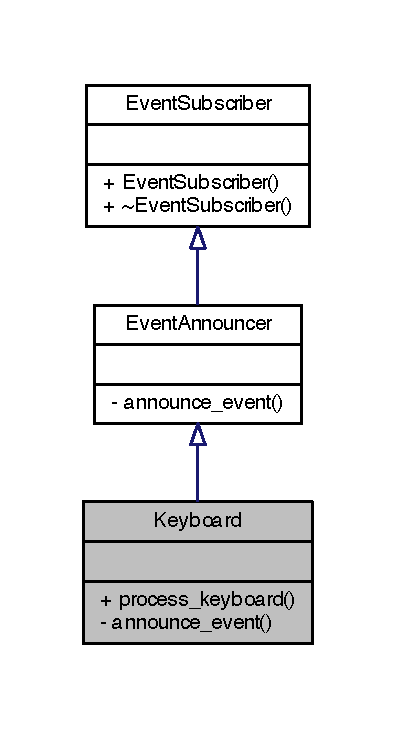
\includegraphics[width=190pt]{class_keyboard__inherit__graph}
\end{center}
\end{figure}


Collaboration diagram for Keyboard\-:
\nopagebreak
\begin{figure}[H]
\begin{center}
\leavevmode
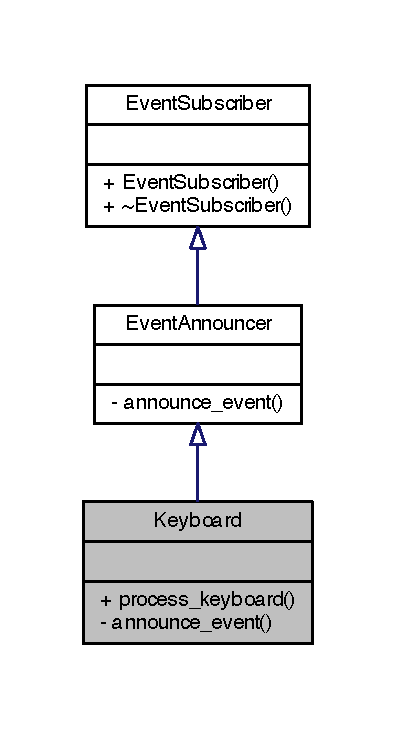
\includegraphics[width=190pt]{class_keyboard__coll__graph}
\end{center}
\end{figure}
\subsubsection*{Public Member Functions}
\begin{DoxyCompactItemize}
\item 
void {\bf process\-\_\-keyboard} ()
\end{DoxyCompactItemize}
\subsubsection*{Private Member Functions}
\begin{DoxyCompactItemize}
\item 
virtual void {\bf announce\-\_\-event} (string key)
\end{DoxyCompactItemize}


\subsubsection{Detailed Description}
Defines class to capture keyboard events and pass them to the processor. 

\begin{DoxyAuthor}{Author}
Alex Cummaudo 
\end{DoxyAuthor}
\begin{DoxyDate}{Date}
19 Oct 2013 
\end{DoxyDate}


\subsubsection{Member Function Documentation}
\index{Keyboard@{Keyboard}!process\-\_\-keyboard@{process\-\_\-keyboard}}
\index{process\-\_\-keyboard@{process\-\_\-keyboard}!Keyboard@{Keyboard}}
\paragraph[{process\-\_\-keyboard}]{\setlength{\rightskip}{0pt plus 5cm}void Keyboard\-::process\-\_\-keyboard (
\begin{DoxyParamCaption}
{}
\end{DoxyParamCaption}
)}\label{class_keyboard_ac2c44b1099dfef44e98ae842140d8338}


Captures keydown events and processes them by passing them to the \doxyref{Event\-Manager}{p.}{class_event_manager}. 

\index{Keyboard@{Keyboard}!announce\-\_\-event@{announce\-\_\-event}}
\index{announce\-\_\-event@{announce\-\_\-event}!Keyboard@{Keyboard}}
\paragraph[{announce\-\_\-event}]{\setlength{\rightskip}{0pt plus 5cm}void Keyboard\-::announce\-\_\-event (
\begin{DoxyParamCaption}
\item[{string}]{key}
\end{DoxyParamCaption}
)\hspace{0.3cm}{\ttfamily [private]}, {\ttfamily [virtual]}}\label{class_keyboard_a95fb72c2a1fc6085f8f76b01e95b97ac}


Sends an event to all subscribers with the given key. 


\begin{DoxyParams}{Parameters}
{\em msg} & Message to announce when creating an \doxyref{Event}{p.}{class_event} \\
\hline
\end{DoxyParams}


Implements {\bf Event\-Announcer} \doxyref{}{p.}{class_event_announcer_a44cb9090f6a15571de9a2f605cd4d898}.



The documentation for this class was generated from the following files\-:\begin{DoxyCompactItemize}
\item 
/\-Users/\-Alex/\-Dropbox/\-Swinburne/\-H\-I\-T2302 -\/ O\-O\-P/\-Projects/\-Cat and Mouse/\#1\-\_\-\-Cat\-Mouse\-\_\-\-C++\-\_\-\-D\-E\-Coupled/src/{\bf Keyboard.\-h}\item 
/\-Users/\-Alex/\-Dropbox/\-Swinburne/\-H\-I\-T2302 -\/ O\-O\-P/\-Projects/\-Cat and Mouse/\#1\-\_\-\-Cat\-Mouse\-\_\-\-C++\-\_\-\-D\-E\-Coupled/src/{\bf Keyboard.\-cpp}\end{DoxyCompactItemize}

\subsection{Log Class Reference}
\label{class_log}\index{Log@{Log}}


{\ttfamily \#include $<$Log.\-h$>$}



Inheritance diagram for Log\-:
\nopagebreak
\begin{figure}[H]
\begin{center}
\leavevmode
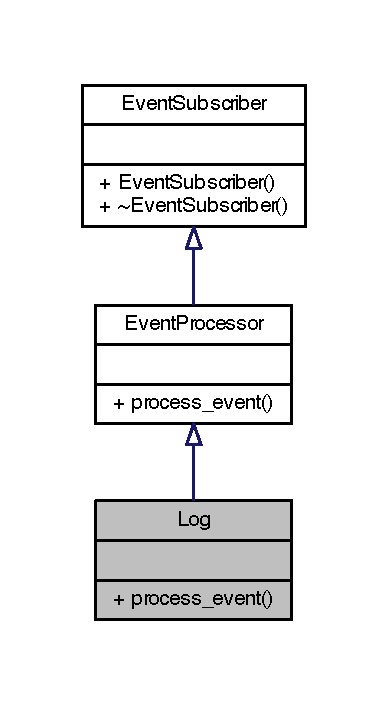
\includegraphics[width=186pt]{class_log__inherit__graph}
\end{center}
\end{figure}


Collaboration diagram for Log\-:
\nopagebreak
\begin{figure}[H]
\begin{center}
\leavevmode
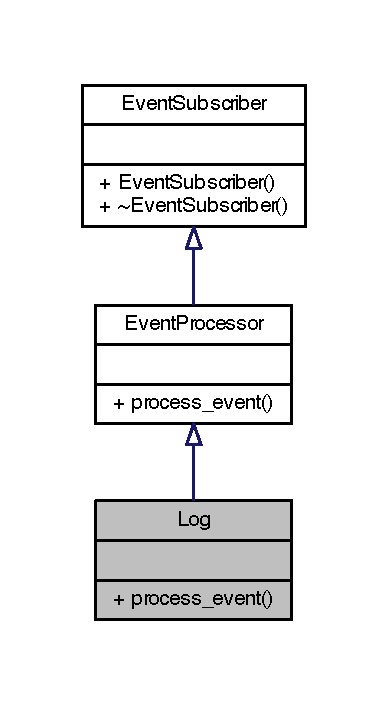
\includegraphics[width=186pt]{class_log__coll__graph}
\end{center}
\end{figure}
\subsubsection*{Public Member Functions}
\begin{DoxyCompactItemize}
\item 
virtual void {\bf process\-\_\-event} ({\bf Event} $\ast$e\-Data)
\end{DoxyCompactItemize}


\subsubsection{Detailed Description}
C\-L\-I view to game. 

\begin{DoxyAuthor}{Author}
Alex Cummaudo 
\end{DoxyAuthor}
\begin{DoxyDate}{Date}
7 Oct 2013 
\end{DoxyDate}


\subsubsection{Member Function Documentation}
\index{Log@{Log}!process\-\_\-event@{process\-\_\-event}}
\index{process\-\_\-event@{process\-\_\-event}!Log@{Log}}
\paragraph[{process\-\_\-event}]{\setlength{\rightskip}{0pt plus 5cm}void Log\-::process\-\_\-event (
\begin{DoxyParamCaption}
\item[{{\bf Event} $\ast$}]{e\-Data}
\end{DoxyParamCaption}
)\hspace{0.3cm}{\ttfamily [virtual]}}\label{class_log_a5be2a1f651af3de38cf26a6a84567f51}


Processes a data depending on the data passed by printing each key/value pair in the event data's map, priting lines to cout. 


\begin{DoxyParams}{Parameters}
{\em e\-Data} & \doxyref{Event}{p.}{class_event} Data to process \\
\hline
\end{DoxyParams}


Implements {\bf Event\-Processor} \doxyref{}{p.}{class_event_processor_a20ce019a16fcf8ba67b6547750bf6655}.



The documentation for this class was generated from the following files\-:\begin{DoxyCompactItemize}
\item 
/\-Users/\-Alex/\-Dropbox/\-Swinburne/\-H\-I\-T2302 -\/ O\-O\-P/\-Projects/\-Cat and Mouse/\#1\-\_\-\-Cat\-Mouse\-\_\-\-C++\-\_\-\-D\-E\-Coupled/src/{\bf Log.\-h}\item 
/\-Users/\-Alex/\-Dropbox/\-Swinburne/\-H\-I\-T2302 -\/ O\-O\-P/\-Projects/\-Cat and Mouse/\#1\-\_\-\-Cat\-Mouse\-\_\-\-C++\-\_\-\-D\-E\-Coupled/src/{\bf Log.\-cpp}\end{DoxyCompactItemize}

\subsection{Mouse Class Reference}
\label{class_mouse}\index{Mouse@{Mouse}}


{\ttfamily \#include $<$Cat\-Mouse.\-hpp$>$}



Inheritance diagram for Mouse\-:
\nopagebreak
\begin{figure}[H]
\begin{center}
\leavevmode
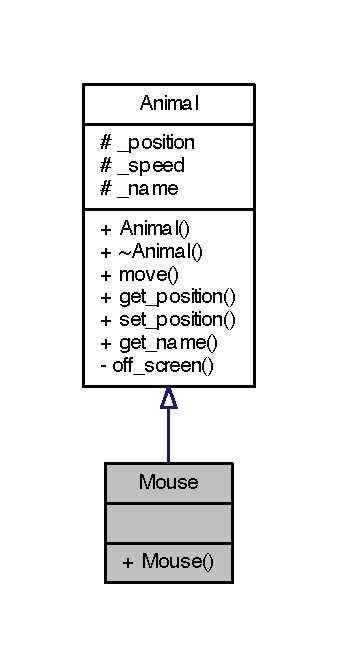
\includegraphics[width=162pt]{class_mouse__inherit__graph}
\end{center}
\end{figure}


Collaboration diagram for Mouse\-:
\nopagebreak
\begin{figure}[H]
\begin{center}
\leavevmode
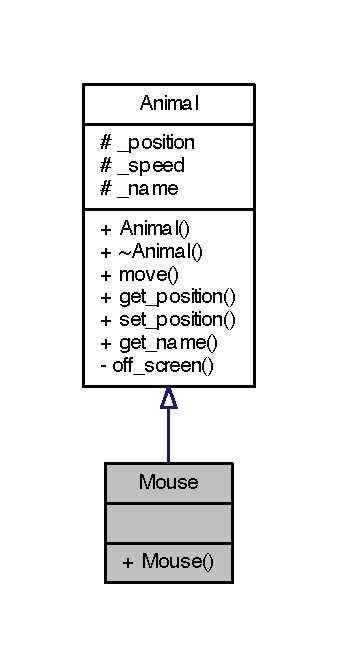
\includegraphics[width=162pt]{class_mouse__coll__graph}
\end{center}
\end{figure}
\subsubsection*{Public Member Functions}
\begin{DoxyCompactItemize}
\item 
{\bf Mouse} ()
\end{DoxyCompactItemize}
\subsubsection*{Additional Inherited Members}


\subsubsection{Detailed Description}
Defines an class for a playable chasee (i.\-e. the hunted mouse) 

\begin{DoxyAuthor}{Author}
Alex Cummaudo 
\end{DoxyAuthor}
\begin{DoxyDate}{Date}
18 Oct 2013 
\end{DoxyDate}


\subsubsection{Constructor \& Destructor Documentation}
\index{Mouse@{Mouse}!Mouse@{Mouse}}
\index{Mouse@{Mouse}!Mouse@{Mouse}}
\paragraph[{Mouse}]{\setlength{\rightskip}{0pt plus 5cm}Mouse\-::\-Mouse (
\begin{DoxyParamCaption}
{}
\end{DoxyParamCaption}
)}\label{class_mouse_a99024d3700d649ae19c1537b42a3e86d}


The default constructor for the mouse constructs parent and sets position on righthand-\/side of screen. 



The documentation for this class was generated from the following file\-:\begin{DoxyCompactItemize}
\item 
/\-Users/\-Alex/\-Dropbox/\-Swinburne/\-H\-I\-T2302 -\/ O\-O\-P/\-Projects/\-Cat and Mouse/\#3\-\_\-\-Cat\-Mouse\-\_\-\-C++\-\_\-\-Coupled/src/{\bf Cat\-Mouse.\-hpp}\end{DoxyCompactItemize}

\subsection{Network Class Reference}
\label{class_network}\index{Network@{Network}}


{\ttfamily \#include $<$Network.\-h$>$}



Collaboration diagram for Network\-:
\nopagebreak
\begin{figure}[H]
\begin{center}
\leavevmode
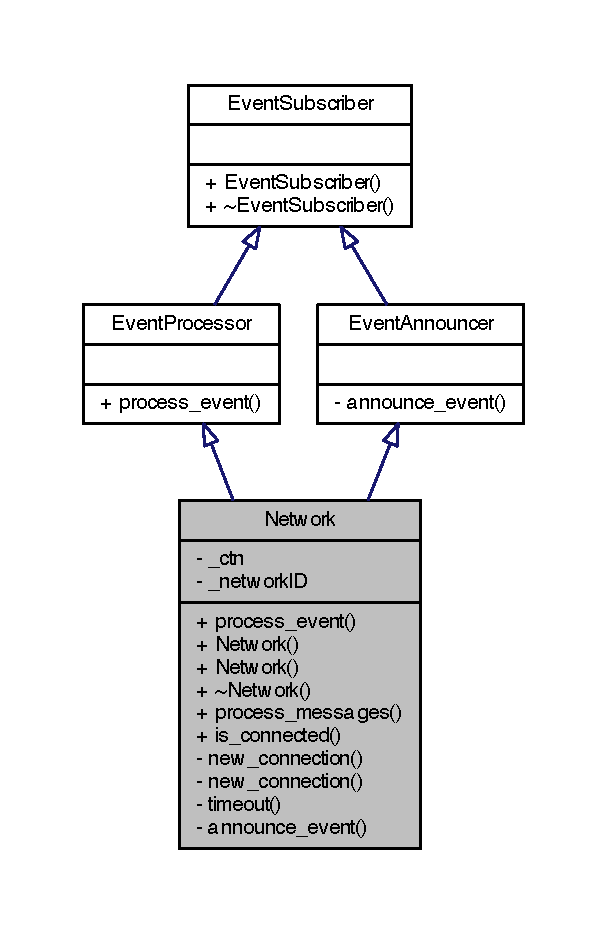
\includegraphics[width=350pt]{class_network__coll__graph}
\end{center}
\end{figure}
\subsubsection*{Public Member Functions}
\begin{DoxyCompactItemize}
\item 
{\bf Network} ({\bf Game} $\ast$game\-Model)
\item 
{\bf Network} ({\bf Game} $\ast$game\-Model, string ip\-Addr)
\item 
{\bf $\sim$\-Network} ()
\item 
void {\bf process\-\_\-messages} ()
\item 
bool {\bf is\-\_\-connected} ()
\item 
void {\bf send\-\_\-message} (string msg)
\end{DoxyCompactItemize}
\subsubsection*{Private Member Functions}
\begin{DoxyCompactItemize}
\item 
connection {\bf new\-\_\-connection} ()
\item 
connection {\bf new\-\_\-connection} (string ip\-Addr)
\item 
void {\bf timeout} (string msg\-Prompt, string msg\-Succ, string msg\-Fail, int timeout\-Secs, function$<$ void(void)$>$ countdown\-Body, function$<$ bool(void)$>$ break\-Condition)
\end{DoxyCompactItemize}
\subsubsection*{Private Attributes}
\begin{DoxyCompactItemize}
\item 
connection {\bf \-\_\-ctn}
\item 
string {\bf \-\_\-network\-I\-D}
\item 
{\bf Game} $\ast$ {\bf \-\_\-game\-Model}
\end{DoxyCompactItemize}


\subsubsection{Detailed Description}
Packages up data recieved from the controller and passes it to a given network. 

\begin{DoxyAuthor}{Author}
Alex Cummaudo 
\end{DoxyAuthor}
\begin{DoxyDate}{Date}
2 Nov 2013 
\end{DoxyDate}


\subsubsection{Constructor \& Destructor Documentation}
\index{Network@{Network}!Network@{Network}}
\index{Network@{Network}!Network@{Network}}
\paragraph[{Network}]{\setlength{\rightskip}{0pt plus 5cm}Network\-::\-Network (
\begin{DoxyParamCaption}
\item[{{\bf Game} $\ast$}]{game\-Model}
\end{DoxyParamCaption}
)}\label{class_network_a43c71b28d82f394c36dfcbab36400883}


Constructor initiates a connection as a host. 


\begin{DoxyParams}{Parameters}
{\em game\-Model} & The game model to link to and update \\
\hline
\end{DoxyParams}
\index{Network@{Network}!Network@{Network}}
\index{Network@{Network}!Network@{Network}}
\paragraph[{Network}]{\setlength{\rightskip}{0pt plus 5cm}Network\-::\-Network (
\begin{DoxyParamCaption}
\item[{{\bf Game} $\ast$}]{game\-Model, }
\item[{string}]{ip\-Addr}
\end{DoxyParamCaption}
)}\label{class_network_ac35ebf94e55df772093a646da958f90b}


Constructor initiates a connection to a given ip address (as a client) 


\begin{DoxyParams}{Parameters}
{\em game\-Model} & The game model to link to and update \\
\hline
{\em ip\-Addr} & The I\-P Address of the host this client will connect to \\
\hline
\end{DoxyParams}
\index{Network@{Network}!$\sim$\-Network@{$\sim$\-Network}}
\index{$\sim$\-Network@{$\sim$\-Network}!Network@{Network}}
\paragraph[{$\sim$\-Network}]{\setlength{\rightskip}{0pt plus 5cm}Network\-::$\sim$\-Network (
\begin{DoxyParamCaption}
{}
\end{DoxyParamCaption}
)}\label{class_network_a7a4e19cdb4bf0c7ecf82baa643831492}


Destructor closes all connections and announces Goodbye message. 



\subsubsection{Member Function Documentation}
\index{Network@{Network}!process\-\_\-messages@{process\-\_\-messages}}
\index{process\-\_\-messages@{process\-\_\-messages}!Network@{Network}}
\paragraph[{process\-\_\-messages}]{\setlength{\rightskip}{0pt plus 5cm}void Network\-::process\-\_\-messages (
\begin{DoxyParamCaption}
{}
\end{DoxyParamCaption}
)}\label{class_network_ad88853109086fc046638ad69b483fbd1}


Process messages that are being recieved (i.\-e. incoming network string to an outgoing event) 

\begin{DoxyNote}{Note}
Any incoming messages that suggests changes to the model will do so directly here. 
\end{DoxyNote}
\begin{DoxyNote}{Note}
Messages recieved in the format\-: key\-:value,key\-:value$|$ etc. Hence we want to parse the msg back into its event kind
\end{DoxyNote}
\index{Network@{Network}!is\-\_\-connected@{is\-\_\-connected}}
\index{is\-\_\-connected@{is\-\_\-connected}!Network@{Network}}
\paragraph[{is\-\_\-connected}]{\setlength{\rightskip}{0pt plus 5cm}bool Network\-::is\-\_\-connected (
\begin{DoxyParamCaption}
{}
\end{DoxyParamCaption}
)}\label{class_network_a825426c85012724d2f41ba4a8e54716e}
Delcare is connected property \begin{DoxyReturn}{Returns}
Boolean whether or not the network is connected 
\end{DoxyReturn}
\index{Network@{Network}!send\-\_\-message@{send\-\_\-message}}
\index{send\-\_\-message@{send\-\_\-message}!Network@{Network}}
\paragraph[{send\-\_\-message}]{\setlength{\rightskip}{0pt plus 5cm}void Network\-::send\-\_\-message (
\begin{DoxyParamCaption}
\item[{string}]{msg}
\end{DoxyParamCaption}
)}\label{class_network_aa5f85cb283b9558262a5605fd68e32b0}


Sends a string over the network by packaging it and sending it over the network as a string (i.\-e. an outgoing event to a network string) 


\begin{DoxyParams}{Parameters}
{\em msg} & String to send over the network \\
\hline
\end{DoxyParams}
\index{Network@{Network}!new\-\_\-connection@{new\-\_\-connection}}
\index{new\-\_\-connection@{new\-\_\-connection}!Network@{Network}}
\paragraph[{new\-\_\-connection}]{\setlength{\rightskip}{0pt plus 5cm}connection Network\-::new\-\_\-connection (
\begin{DoxyParamCaption}
{}
\end{DoxyParamCaption}
)\hspace{0.3cm}{\ttfamily [private]}}\label{class_network_ae4d9e6c18f9569f5fbc6812b3f425b2e}


Initiates the connection as a host, returning true or false on a success or error. 

\begin{DoxyReturn}{Returns}
A new host connection to work with 
\end{DoxyReturn}
Force break condition to be true \index{Network@{Network}!new\-\_\-connection@{new\-\_\-connection}}
\index{new\-\_\-connection@{new\-\_\-connection}!Network@{Network}}
\paragraph[{new\-\_\-connection}]{\setlength{\rightskip}{0pt plus 5cm}connection Network\-::new\-\_\-connection (
\begin{DoxyParamCaption}
\item[{string}]{ip\-\_\-addr}
\end{DoxyParamCaption}
)\hspace{0.3cm}{\ttfamily [private]}}\label{class_network_a8a6b29f8675b35819073f0fa388e7b37}


Initiates the connection as a client, returning true or false on a success or error. 


\begin{DoxyParams}{Parameters}
{\em ip\-\_\-addr} & I\-P Address that this client should connect to \\
\hline
\end{DoxyParams}
\begin{DoxyReturn}{Returns}
A new client connection to work with 
\end{DoxyReturn}
\index{Network@{Network}!timeout@{timeout}}
\index{timeout@{timeout}!Network@{Network}}
\paragraph[{timeout}]{\setlength{\rightskip}{0pt plus 5cm}void Network\-::timeout (
\begin{DoxyParamCaption}
\item[{string}]{msg\-Prompt, }
\item[{string}]{msg\-Succ, }
\item[{string}]{msg\-Fail, }
\item[{int}]{timeout\-Secs, }
\item[{function$<$ void(void)$>$}]{countdown\-Body, }
\item[{function$<$ bool(void)$>$}]{break\-Condition}
\end{DoxyParamCaption}
)\hspace{0.3cm}{\ttfamily [private]}}\label{class_network_a1368ca33ad5eec63f5146c878756a08b}


The timeout connection; runs the passed function success on a success, and error function on error; allow passing of two functors so that lambda expressions can be passed in as parameters to the timeout. 


\begin{DoxyParams}{Parameters}
{\em msg\-Prompt} & Prompt message announced when timeout begins (i.\-e., why we're having a timeout). \\
\hline
{\em msg\-Succ} & Message announced when timeout did not run out and the break condition was met \\
\hline
{\em msg\-Fail} & Message announced when timeout did ran out of timeout\-Secs and the break condition was never met \\
\hline
{\em timeout\-Secs} & How long to run timeout for \\
\hline
{\em countdown\-Body} & Function to run every second on timeout \\
\hline
{\em break\-Condition} & Function that returns a bool to check whether or not the timeout should break \\
\hline
\end{DoxyParams}


\subsubsection{Member Data Documentation}
\index{Network@{Network}!\-\_\-ctn@{\-\_\-ctn}}
\index{\-\_\-ctn@{\-\_\-ctn}!Network@{Network}}
\paragraph[{\-\_\-ctn}]{\setlength{\rightskip}{0pt plus 5cm}connection Network\-::\-\_\-ctn\hspace{0.3cm}{\ttfamily [private]}}\label{class_network_a86ac539e91f6178d7f3435e65e406dc0}


\doxyref{Network}{p.}{class_network} connection controller between client and host. 

\index{Network@{Network}!\-\_\-network\-I\-D@{\-\_\-network\-I\-D}}
\index{\-\_\-network\-I\-D@{\-\_\-network\-I\-D}!Network@{Network}}
\paragraph[{\-\_\-network\-I\-D}]{\setlength{\rightskip}{0pt plus 5cm}string Network\-::\-\_\-network\-I\-D\hspace{0.3cm}{\ttfamily [private]}}\label{class_network_aa2745126e6c7593e849e9522fdcc3b54}


Defines a unique address of this machine. 

\index{Network@{Network}!\-\_\-game\-Model@{\-\_\-game\-Model}}
\index{\-\_\-game\-Model@{\-\_\-game\-Model}!Network@{Network}}
\paragraph[{\-\_\-game\-Model}]{\setlength{\rightskip}{0pt plus 5cm}{\bf Game}$\ast$ Network\-::\-\_\-game\-Model\hspace{0.3cm}{\ttfamily [private]}}\label{class_network_a462a3d6a72eb7cf8c7a1db32dfc527e0}


Defines the coupling between game and network. 



The documentation for this class was generated from the following files\-:\begin{DoxyCompactItemize}
\item 
/\-Users/\-Alex/\-Dropbox/\-Swinburne/\-H\-I\-T2302 -\/ O\-O\-P/\-Projects/\-Cat and Mouse/\#3\-\_\-\-Cat\-Mouse\-\_\-\-C++\-\_\-\-Coupled/src/{\bf Network.\-h}\item 
/\-Users/\-Alex/\-Dropbox/\-Swinburne/\-H\-I\-T2302 -\/ O\-O\-P/\-Projects/\-Cat and Mouse/\#3\-\_\-\-Cat\-Mouse\-\_\-\-C++\-\_\-\-Coupled/src/{\bf Network.\-cpp}\end{DoxyCompactItemize}


\end{document}
